\chapter{Introduction}
\label{chp:intro}
Intelligent robots are becoming increasingly important in both industry and everyday life. In industry, rising labor costs are motivating manufacturers to consider using more robots in factories. For example, when the average minimum wage in China has increased by more than 20 percent in 2012, the supply of manufacturing robots has also increased by 51 percent in China~\cite{IFR:report}. 
Europe and USA exhibit similar trends: Intelligent robots are being designed in order to make workers more productive and make manufacturers more competitive in terms of price and quality. Among these intelligent robots is the new ``Baxter'' robot~\cite{Brooks:2012:Baxter}, which is equipped with software that enables the robot to learn various tasks, recognize different objects, and react intelligently to external forces. Intelligent robots are expected to assist people in everyday life. In the future, such robots are expected to perform various tasks, including 1) household and care support, such as cooking and laundry; 2) healthy life support, such as chatting with the elderly and taking care of people with disabilities; and 3) labor support in unsafe working conditions such as chemical plants~\cite{Yamazaki:2012}. Several successful prototypes for assistant robots exist. For example, the PR2 robot from Willow Garage$^\copyright$ has been shown to assist people with severe physical disabilities such as quadriplegia~\cite{PR2HumanityWeb}; humanoid robots such as the HPR-4 can perform human-like actions and can communicate with people using speech~\cite{HRP-Cyber}. In addition to their applications in industry and everyday life, modern intelligent robots can be helpful in other areas, including autonomous vehicles~\cite{Montemerlo:2008:JSE}, medical and surgical intervention ~\cite{Bonfe:2012}, emergency and disaster rescue~\cite{Fukushima:2011}, and military tasks~\cite{AlphaDog:2012}.



\begin{figure}[htb]
  \centering
  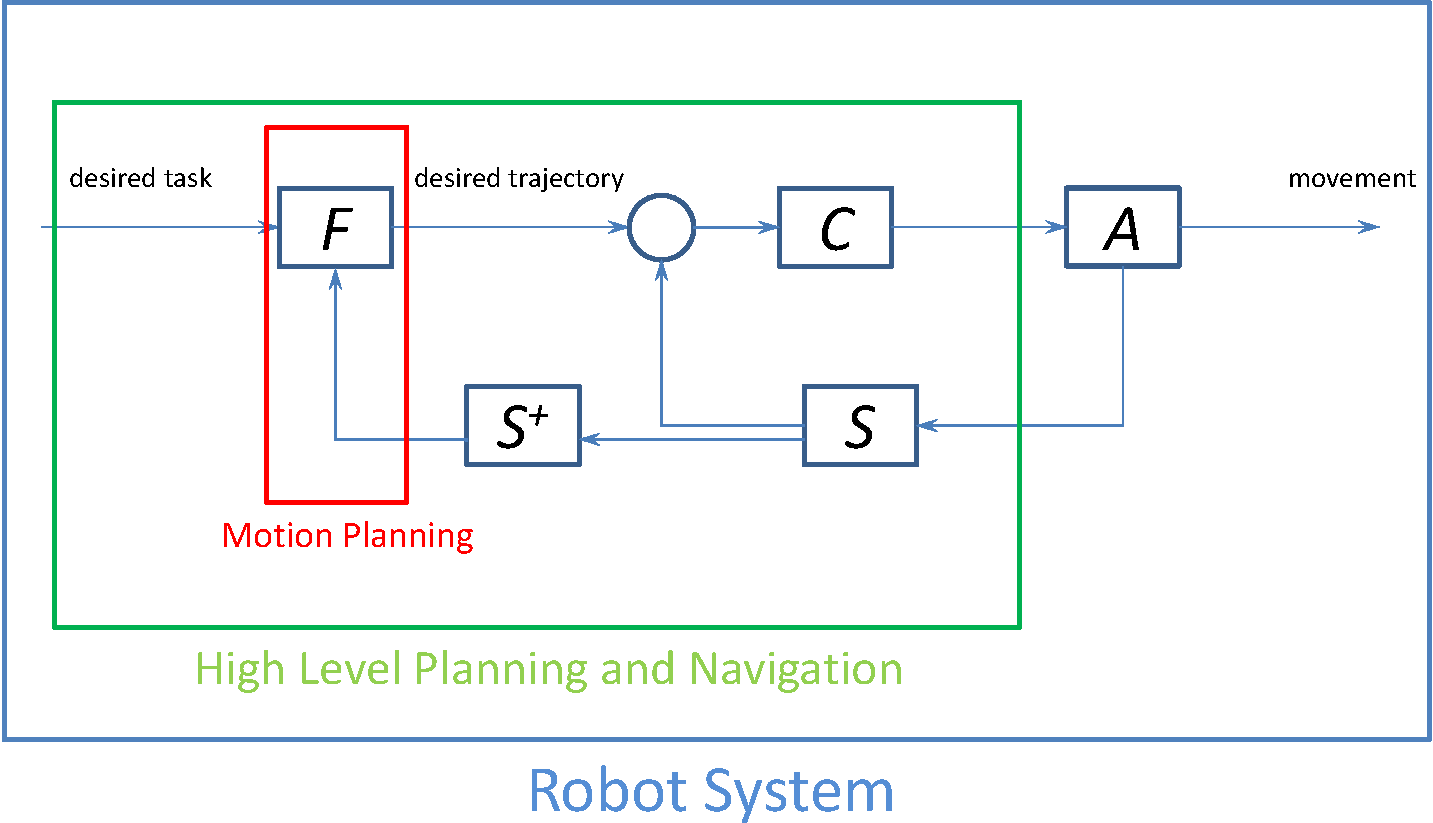
\includegraphics[width=\linewidth]{figs/1/pipeline-crop.pdf}
  \caption[Important hardware and software subsystems in a robot system]{Important hardware and software subsystems in a robot system. 1) Feed-forward system (F), including task planning, navigation strategy, motion planning and trajectory generation. 2) Control system (C), including kinematics, dynamics and control algorithms. 3) Actuator system (A), including motors, servos, transmissions and so forth. 4) Sensor system (S), including various sensors such as camera, laser, IMU and related low level sensor data processing algorithms such as signal processing, estimation and fusion. 5) Sensor post-processing system (S$^+$), including localization, mapping, etc. The main software component of a robot system is the \emph{high level planning and navigation}, which determines the instructions sent to the actuator system, given the desired tasks to be executed. One important component of high level planning and navigation is \emph{motion planning}, which focuses on computing the trajectory from the environment description.}
  \label{fig:1:pipeline}
\end{figure}

The tremendous improvement in the design and availability of intelligent robots over the last decade is based on progress in many related areas, including computer vision, artificial intelligence, machine learning, control, sensor systems, and mechanical systems, which correspond to different components of an intelligent robot system (Figure~\ref{fig:1:pipeline}). For example, the SLAM (simultaneous localization and mapping) algorithm enables a robot to accurately track its position in an unknown environment~\cite{PR:2005}. In addition, with the help of advanced vision techniques, robots can now recognize and segment objects from background point clouds~\cite{Rusu:2009:IROS}. 
Compared to traditional industrial robots, one important feature of the modern intelligent robot system is \emph{high level planning and navigation}. Its main purpose is to compute low-level instructions based on high level descriptions for the tasks to be executed; these low-level instructions are then provided to the robot actuator system.
This component is composed of many different sub-components (Figure~\ref{fig:1:pipeline}) and there has been extensive work in this area, such as task planning~\cite{LPT:TPP:1989}, feedback from observation~\cite{KLP:2012:UPE,KLP:2011:NOW}, optimal control~\cite{Stengel:1994:OC}, and adaptive control~\cite{Astrom:1994:AC}.


One of the most important sub-systems of the high level planning and navigation component is the \emph{motion planning} system, which enables the robot to move safely from an initial position to a goal position without colliding with any static or moving obstacles in the environment. Motion planning enables robots to work efficiently and reliably in dynamic environments along with humans. Motion planning problems can be directly formalized and solved in the 3D workspace, for instance with the widely-used potential field algorithms~\cite{Khatib:IJRR:1986}. However, these workspace solutions cannot easily handle robots with different geometries and mechanical constraints. To overcome these difficulties, 
motion planning may be formalized and solved in a new space called the \emph{configuration space}~\cite{Lozano-Perez:1979:APC,LPT:APM:1981,LPT:SpatialPlanning:1983}. In the configuration space, a robot with a complex geometric shape in 3D workspace is mapped to a point robot and the robot's trajectory will correspond to a continuous curve in the high-dimensional configuration space (Figure~\ref{fig:1:planning}). Based on the configuration space formulation, the motion planning problem can be solved in two steps:

\begin{enumerate}
\item Construct a representation of the configuration space.
\item Perform optimization based on the computed representation.
\end{enumerate}

This motion planning pipeline based on configuration spaces is very successful and is adopted by many real-world planning applications that require optimal planning solutions. Many different representations for the configuration space have been proposed, including polyhedrons~\cite{Chazelle:ADS:1987}, semi-algebraic sets~\cite{Canny:1988:AGC,Canny:1988:CKP}, graphs~\cite{Kavraki96}, and trees/forests~\cite{Kuffner00}. Different optimization approaches have been proposed for different configuration space representations, including computing a shortest path, computing the minimum distance to the boundary of a closed set inside the configuration space and so forth. Moreover, the same pipeline is also implicitly used in some motion planning algorithms for only computing a feasible path (i.e., a collision-free path that does not violate other constraints). For example, many variants of Rapidly Exploring Random Tree (RRT)~\cite{Kuffner00} use different heuristics to guide the search toward the goal configuration while growing a search tree structure as an approximate representation of the configuration space. Such a strategy can be viewed as a variant of the above pipeline, in which the configuration space construction alternates with the optimization computation.


However, this $\Cspace$-based pipeline still has many challenges:
\begin{enumerate}
\item Efficiently compute an approximate or exact representation for the configuration space is difficult, especially for high-DOF robots with high-dimensional configuration spaces. Such problem would have exponential complexity (Section~\ref{sec:1:configconstruction}).
\item Many robotics applications require real-time planning in order to work reliably and efficiently in human environments with moving obstacles, but performing optimization in the computed representation for the configuration space can be time consuming (Section~\ref{sec:1:optimization}).
\item A robot in the real world depends on various sensors to acquire knowledge about its own state and the surrounding environments. Since the sensors provide noisy data, one important open problem involves enhancing the configuration space to consider robots and environments with noisy geometries. In contrast, previous work on configuration space based computations assume an exact representation of the robot and obstacles (Section~\ref{sec:1:uncertainty}).
\end{enumerate}


\section{Configuration Space}
\label{sec:1:configurationSpace}
The configuration space is a key concept used in classical mechanics to describe and analyze the motion of many important systems~\cite{Arnold:1989}. Generally, a \emph{configuration} $\q$ is a vector of independent parameters uniquely specifying the state of a system; a configuration space or $\Cspace$ is a collection of all possible configurations for a given system. For example, for a system of $n$ point particles, the configuration is a vector describing the positions of all the particles and the corresponding $\Cspace$ is $\mathbb R^{3n}$; the configuration of a 3D rigid body consists of its position and orientation, and the configuration space is $\SEcubic$ is both rotation and translation are allowed, and $\Rcubic$ if only translation is allowed; the configuration of an articulated object is the vector of all its joint angles.

The configuration space of a robot $A$ is composed of two components: \emph{collision-free space} $\Cfree = \{\q: A(\q) \cap B = \emptyset\}$ and \emph{in-collision space} or \emph{obstacle space} $\Cobs = \{\q: A(\q) \cap B \neq \emptyset\}$, where $B$ is the geometry for obstacles in the environment and $A(\q)$ corresponds to $A$ with the configuration $\q$. $\Cobs$ is a closed set and its boundary is denoted as the \emph{contact space} $\Ccont = \partial \Cobs$, which corresponds to the set of configurations where $A$ and $B$ just touch each other without penetration. Figure~\ref{fig:1:contactspace} shows an example of the $\Cspace$ of two objects where $\Ccont$ is highlighted with orange curves.

\begin{figure}[htb]
  \centering
  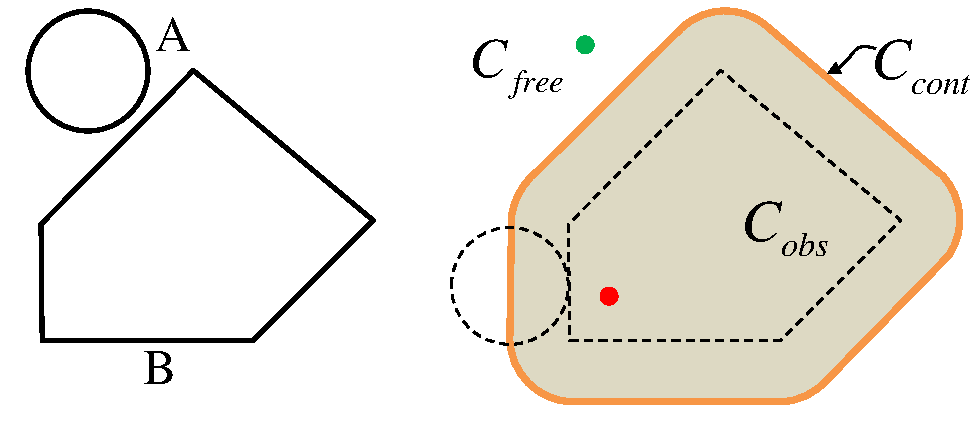
\includegraphics[width=0.6\linewidth]{figs/1/Ccont.pdf}
  \caption[The configuration space of two objects]{The configuration space of two objects. The orange curve highlights the contact space $\Ccont$ of A and B. A point inside/on the orange curve belongs to
  $\Cobs$ and a point outside the orange curve belongs to $\Cfree$.
  The red and green points denote configurations in $\Cobs$ and $\Cfree$, respectively. Intuitively, $\Ccont$ is the boundary that separates in-collision and collision-free configurations.}
  \label{fig:1:contactspace}
\end{figure}

In the special case when $A$ and $B$ are both rigid objects and robot $A$ can only perform translation motion, $\Cobs$ is equal to the well-known Minkowski sum between $A$ and $B$: $\Cobs = A \oplus (-B) = \{\x = \x_A + \x_B | \x_A \in A, \x_B \in -B \}$. One example of the Minkowski sum is shown in Figure~\ref{fig:1:contactspace}. When robot $A$ can perform general motion (i.e., both translation and rotation), the geometry of $\Cobs$ is much more complicated, as shown by the 2D example in Figure~\ref{fig:1:cspaceSE2}.

\begin{figure}[htb]
  \centering
  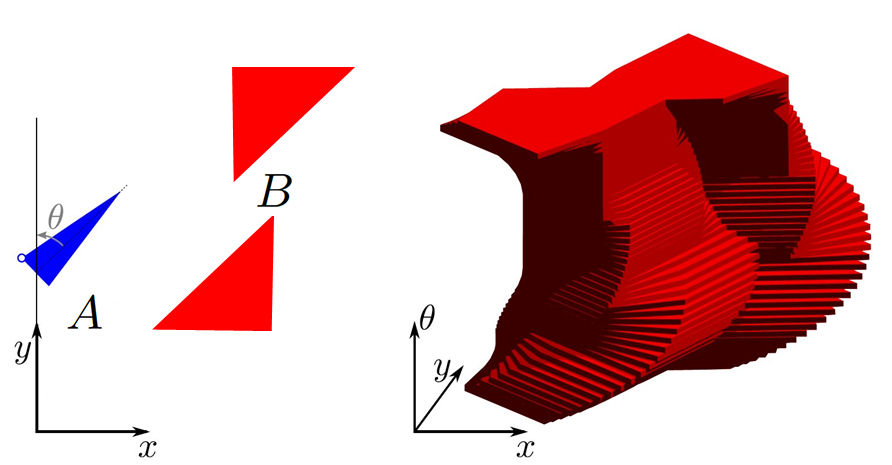
\includegraphics[width=0.9\linewidth]{figs/1/cspaceSE2.png}
  \caption[$\Cobs$ between 2D rigid objects $A$ and $B$]{$\Cobs$ between 2D rigid objects $A$ and $B$. For each rotation angle $\theta \in [0, 2\pi)$, we can compute the Minkowski sum between $A(\theta)$ and $-B$, where $A(\theta)$ is the resulting shape after rotating $A$ about the origin with $\theta$ degrees. When stacking the Minkowski sums for all angles $\theta$, we obtain the $\Cobs$ between $A$ and $B$. This figure is modified from an online image with unknown source.}
  \label{fig:1:cspaceSE2}
\end{figure}

Based on the notion of configuration space, the motion planning problem in 3D workspace can be reduced to path planning for a point robot in $\Cspace$, i.e., finding a curve in $\Cfree$ connecting the given initial and goal configurations of the robot.

\section{Configuration Space Construction}
\label{sec:1:configconstruction}
Before performing the motion planning computation in the configuration space, one prerequisite is to compute the geometry of $\Cspace$ in an appropriate representation (e.g., a graph or a surface). Since $\Cspace = \Cfree \cup \Cobs$ and $\Cfree \cap \Cobs = \emptyset$, we only need to construct the representation for either $\Cfree$ or $\Cobs$. Another equivalent solution is to compute $\Ccont$, the boundary between $\Cfree$ and $\Cobs$.

Previous work on configuration space construction can be categorized into two different methods: geometry-based and topology-based. Geometry-based methods compute the exact geometric representation of the configuration space while topology-based methods capture the connectivity of the configuration space.

Geometry-based methods are usually limited to low-dimensional configuration spaces, due to the combinatorial complexity involved in computing the boundary of $\Cobs$ for high-dimensional configuration spaces. Most previous work has focused on the special case when objects $A$ and $B$ are rigid bodies only performing translational motion. As mentioned in Section~\ref{sec:1:configurationSpace}, the resulting $\Cobs$ is the Minkowski sum between $A$ and $-B$. Even for this special case, the computational complexity involved in computing $\Cobs$ is still high: the complexity is $\mathcal O(mn)$ when $A$ and $B$ are both convex-objects and is $\mathcal O(m^3n^3)$ when $A$ and $B$ are both non-convex objects~\cite{Halperin:2002:RGC}, where $m$ and $n$ are the number of triangles in $A$ and $B$, respectively. In addition to the high complexity, most existing implementations for computing the Minkowski sum are prone to challenges that arise in the context of 3D geometric algorithms. In particular, these implementations are 1) not robust to numerical error, 2) susceptible to degeneracies (i.e., cannot reliably handle polygon soups or meshes with holes). Recent work has proposed methods~\cite{Lien:2008:CMS,Lien:2007:ACD,Lien:2009:ASM} for computing the approximate Minkowski sum efficiently and reliably, but these methods are also prone to robustness issues and can have high complexity in terms of dealing with complex objects. Options other than the Minkowski sum exist for computing  $\Cobs$. For example, Varadhan et al. compute the $\Cobs$ for 2D objects with rotation and translation by approximating the $\Cobs$ with an adaptive grid~\cite{Varadhan:2006:TPA}; Zhang et al. compute an approximation to 4-D $\Cspace$ using cell decomposition~\cite{Zhang:2007:IROS}.

Topology-based methods capture the connectivity of the configuration space. Most previous approaches attempt to capture the connectivity of $\Cfree$ using sampling techniques~\cite{Kavraki96,Kuffner00}. The basic idea is first to generate random samples (called milestones) in $\Cfree$ and then organize these samples using a graph structure or a forest of tree structures (Figure~\ref{fig:1:topologycspace}). As the topology of $\Cfree$ can be rather complex, and
may consist of multiple components or small, narrow passages, it is hard to capture the full connectivity of $\Cfree$ using random sampling. There is extensive work on improving the connectivity computation by using different sampling strategies~\cite{Amato:1998:OOP,Boor:1999:ICRA,Hsu:1998:FNP,Rodriguez:2006,Zhang:2008:ICRA,Zheng:2005}. Recent work attempts to capture the topology of both $\Cfree$ and $\Cobs$~\cite{Jory:2011:IROS}. Topology-based methods can compute an approximate $\Cspace$ representation much faster than geometry-based methods. However, these methods do not work well with narrow passages and can be slow for high-DOF robots.


\begin{figure}[htb]
  \centering
  \subfloat[Graph representation]{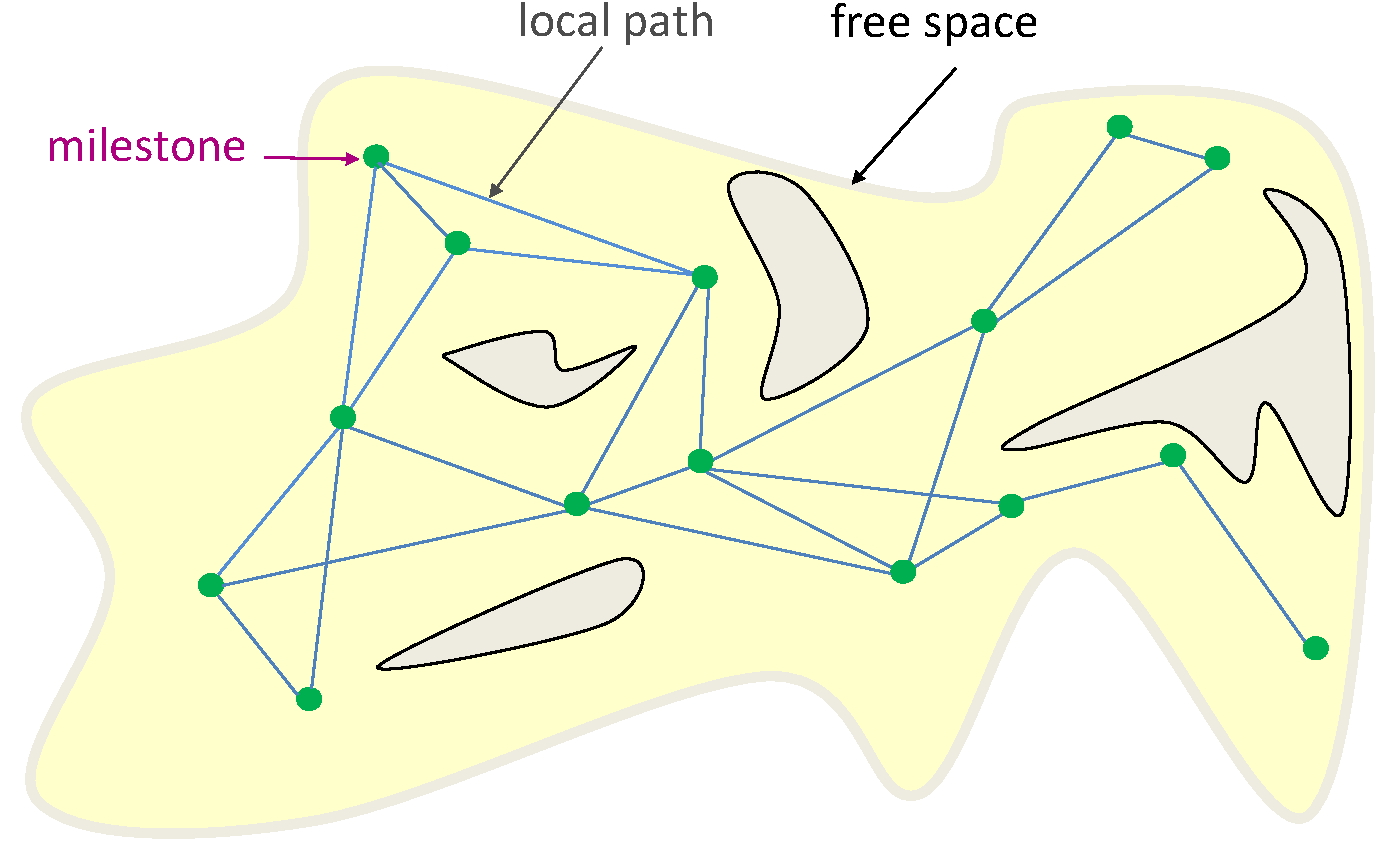
\includegraphics[width=0.49\linewidth]{figs/1/topology1.pdf}}
  \subfloat[Tree representation]{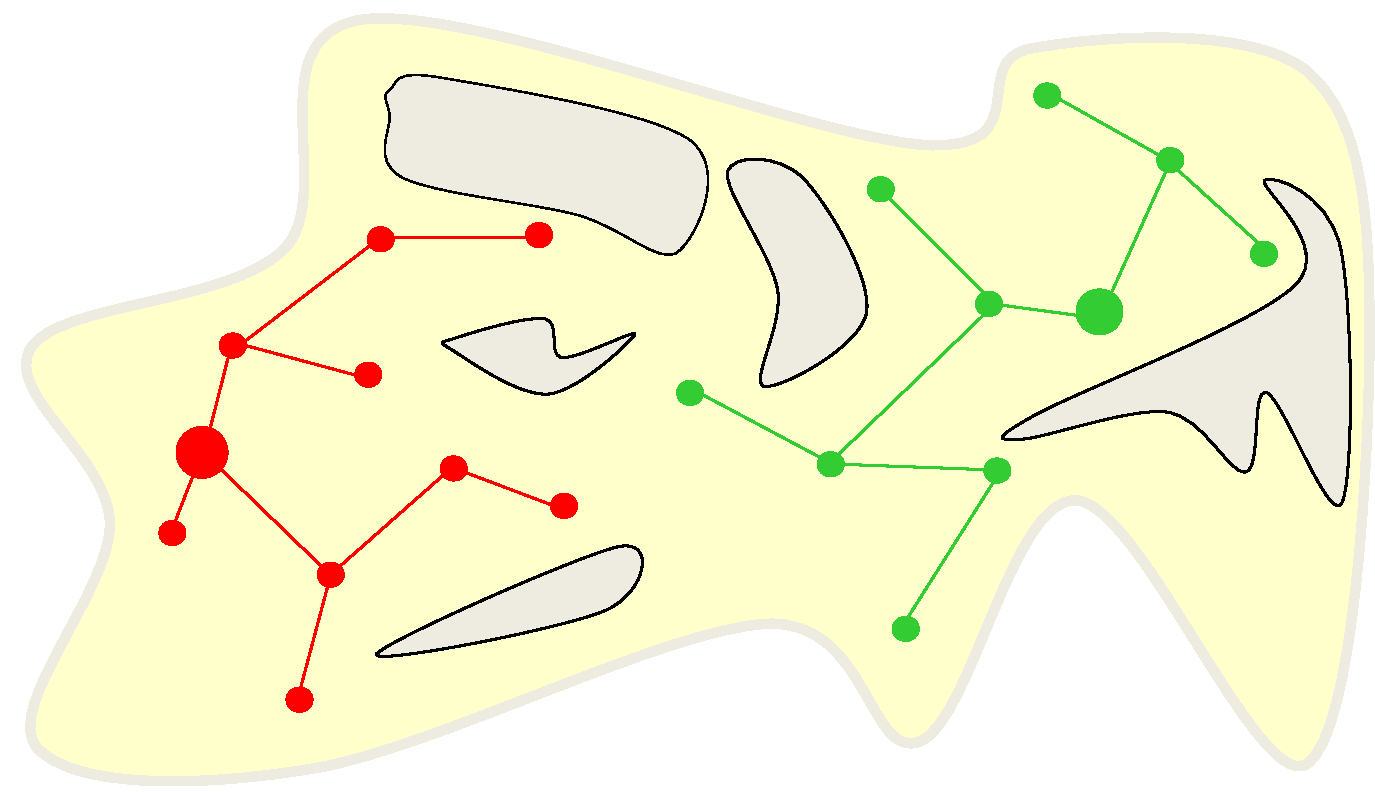
\includegraphics[width=0.49\linewidth]{figs/1/topology2.pdf}}
  \caption[Topology-based methods for configuration space computation]{Topology-based methods for configuration space computation. (a) Capture $\Cfree$ using a graph structure. (b) Capture $\Cfree$ using a forest of tree structures. The two figures are modified from Jean-Claude Latombe's lecture slides.}\label{fig:1:topologycspace}
\end{figure}




\section{Optimization in Configuration Space}
\label{sec:1:optimization}
Once an exact or approximate representation for the configuration space is computed, we next need to perform optimization in this $\Cspace$ representation. For example, the goal motion planning is to compute a trajectory in $\Cspace$, as shown in Figure~\ref{fig:1:planning}. The trajectory should satisfy the following constraints: 1) it should be completely inside $\Cfree$; 2) it should be feasible, e.g., for humanoid robots, the robot should not fall down when following the trajectory. Moreover, 
it is preferable for the trajectory to be optimal under some metric. For instance, the optimal trajectory could be the shortest, take the least time to execute, or maintain the maximum distance from obstacles.
As a result, motion planning can be formalized as a constrained optimization problem in $\Cspace$. Similar formulation can be applied to different applications, such as penetration depth computation~\cite{Zhang:2007:GPD,Zhang:2007:AFP,Zhang:2008:ICRA,Je:2012:PRP}.


\begin{figure}[htb]
  \centering
  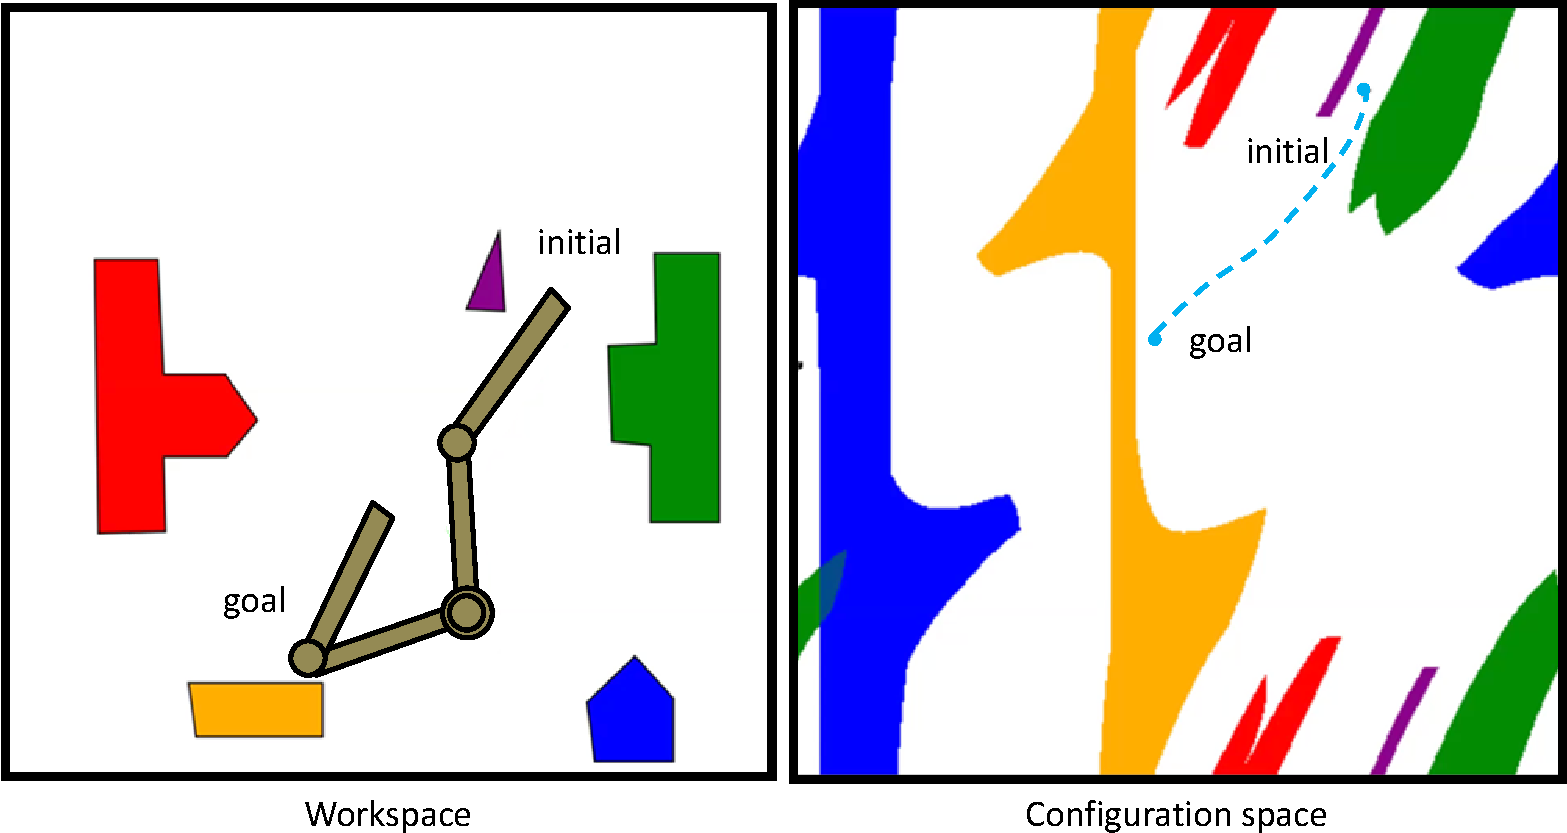
\includegraphics[width=\linewidth]{figs/1/planning-crop.pdf}
  \caption[Motion planning in workspaces and in configuration spaces]{Motion planning in workspaces and in configuration spaces. The left figure shows obstacles (with different colors) and a 2-linked robot in the workspace (both the initial and goal settings). The right figure shows the configuration space corresponding to the workspace in the left figure, where different colors describe the correspondence between obstacles in the workspace and obstacles in the configuration space. The blue curve is a trajectory connecting the initial and goal configurations, and is the result of motion planning algorithm. This figure is modified from~\cite{cspaceJapplet}. \label{fig:1:planning}}
\end{figure}


Optimization in $\Cspace$ is usually computationally expensive, especially for a high-dimensional $\Cspace$ with a complicated structure and topology. To illustrate the computational challenge for $\Cspace$ optimization problems, we take motion planning in $\Cspace$ as an example. Theoretically, motion planning using the exact representation of $\Cspace$ has high computational complexity. Planning algorithms are considered to be `complete' if for any planning problem instance, the algorithm will either find a solution or will correctly report that no solutions exists. Complete planning algorithms have been proved to be PSPACE-hard~\cite{Reif:1979:CMP} and PSPACE-complete~\cite{Canny:1988:AGC}, and kinodynamic motion planning (i.e., motion planning with simple kinematic/dynamic constraints) has been shown to be NEXPTIME-hard~\cite{Canny:1988:CKP}. 
The decidability is still unknown for motion planning with general differential constraints~\cite{Cheng:2007:DMP}. When the approximate representation of $\Cspace$ is used (e.g., using a graph or forest to approximate the connectivity of $\Cfree$), there exist approximate motion planning algorithms that provide guarantees of probabilistic completeness~\cite{Kavraki96,Kuffner00} and/or asymptotic optimality~\cite{Sertac:IJRR:2011}. The complexity of these approximate motion planning algorithms is usually bounded by $\mathcal O(n\ln n)$ where $n$ is the number of configuration samples used in the approximate representation of $\Cspace$.Since $n$ can be very large when $\Cfree$ has narrow passages and/or high dimensionality~\cite{Hsu:2006:ijrr}, the performance of these approximate algorithms is still far from real-time.

Various planning methods related with $\Cspace$ have been proposed in the past decades, including optimization-based planning algorithms such as CHOMP~\cite{Ratliff:2009} and search-based algorithms such as Anytime A*~\cite{Likhachev05anytimedynamic}. For motion planning of high-DOF (degrees-of-freedom) robots, most of the practical methods are based on randomized algorithms, including Probabilistic Roadmap (PRM)~\cite{Kavraki96} and Rapidly Exploring Random Tree (RRT)~\cite{Kuffner00}.


\section{Uncertainty Modeling in Configuration Space}
\label{sec:1:uncertainty}
Most prior techniques assume that an exact geometric representation is known for the robot and obstacles in the environment. This is reasonable in applications such as computer graphics, CAD, and simulation, where the geometric representation of synthetic objects is available. As a result, there is no ambiguity about the collision status of any configuration $\mathbf q \in \Cspace$: either $\q \in \Cfree$ and is collision-free or $\q \in \Cobs$ and is in-collision.

Unfortunately, this exact geometric representation assumption may not hold when we are dealing with real-world robots that interact with the physical environment. In the real world, sensors do not provide exact geometric representation, but rather noisy point clouds. The noise may arise from device noise, limited field-of-view, sensor refresh latency, synchronization error, or even occlusions. For noisy geometric representations, we cannot deterministically compute the collision status of a given configuration $\q$. Instead, $\q$ may lie in $\Cfree$ with probability $p$ and lie in $\Cobs$ with probability $1-p$, where $0 \leq p \leq 1$. Computing $p$ for any configuration $\q \in \Cspace$ is an open problem not studied in previous work.

The problem of modeling uncertainty in the configuration space has many applications. For example, it can be combined with motion planning algorithms to compute a trajectory that minimizes the probability to collide with the obstacles, which would improve the safety of robot navigation. Moreover, it can extend classical computational geometry algorithms to handle noisy sensor data, such as Minkowski sums~\cite{Varadhan:2006:TPA} and offsets~\cite{Choi:1997:CAD}.

\section{Thesis Statement}

Our thesis is as follows:

\textit{High-dimensional configuration spaces can be efficiently approximated using machine learning and geometric algorithms, and used for optimization queries related to motion planning and proximity computations on exact and noisy datasets.}

\section{Main Results}
In support of our thesis, we present new techniques for configuration space construction, optimization computation in configuration spaces, and modeling uncertainty in configuration spaces. First, we demonstrate how to convert the configuration space construction problem into a machine learning problem, and then use active learning to compute an approximate configuration space efficiently and robustly. We also discuss how to use instance-based learning techniques to incrementally compute an approximate configuration space, which enables robots to learn from their past experiences about task execution. Second, we provide parallel GPU-based algorithms to accelerate the optimization computations in the configuration space, which can allow for real-time planning computation in many challenging environments. Finally, we propose two different methods to model the uncertainty in the configuration space caused by noisy geometries. These two methods are then combined with active sensing techniques to enable robots to work reliably in environments with uncertainty.

\subsection{Efficient $\Cspace$ Construction}
In this part, we describe two different methods to compute approximate representation of the configuration space. The first is a geometry-based method and the second is a topology-based method.

First, we present a novel technique to efficiently approximate $\Ccont$ between two rigid objects using machine learning techniques. We first generate a set of samples in $\Cspace$ using collision detection techniques. We use non-linear SVM-based regression to construct an initial (coarse) approximation of $\Ccont$. Then we use active learning techniques to refine this approximation so that it is close enough to the actual $\Ccont$. We provide error bounds on the learned approximate $\Ccont$ and evaluate performance on many complex benchmarks. Additionally, based on the computed configuration space, we present an algorithm to efficiently approximate the penetration depth between two rigid objects, which is important in physically-based simulation.

Second, we present a novel approach to incrementally construct an approximate representation of $\Cspace$ from the samples generated during prior executions of the planning algorithm. Our formulation stores the results of prior collision queries and local planning queries. This information is used to accelerate the performance of planners. We present fast and novel algorithms to perform $\knn$ ($k$-nearest neighbor) queries in high dimensional $\Cspace$ and derive tight bounds on their accuracy. Our approach is general, makes no assumptions about the sampling scheme, and can be used with various sample-based motion planners with only small changes to these planners. Additionally, we discuss how to use this method to enable the planner to learn from its past query instances.

\subsection{Efficient Optimization in $\Cspace$}
In this part, we present techniques to accelerate optimization computation in $\Cspace$ using capabilities of many-core GPUs. This includes a GPU-based parallel planning algorithm called g-Planner. In g-Planner, GPU improves performance by addressing two main bottlenecks of sample-based planning algorithms: collision detection and $k$-nearest neighbor search, which can take more than 95\% of the overall planning time. We present a new GPU-based parallel collision detection
algorithm, which is able to efficiently handle a large number (i.e., more than 100,000) of collision queries between objects of varying complexity and runs more than 60 times faster than single-core CPU
algorithms. For $\knn$ search queries, we describe a new approximate algorithm for $\knn$ search based on Locality-Sensitive
Hashing (LSH), which is a GPU-friendly algorithm with sub-linear complexity and bounded error. The resulting
parallel GPU-based $\knn$ is at least 50 times faster than the optimized single-core CPU implementation.

\subsection{Uncertainty Modeling in $\Cspace$}
In order to model configuration spaces for noisy geometric representations, we first discuss a probabilistic collision detection algorithm between two objects represented as noisy point clouds. We convert the collision problem into a two-class classification problem and use extended SVM algorithms to solve it. To improve efficiency, a divide-and-conquer method is used to eliminate unnecessary computations. Instead of only the binary result (i.e., collision or not) provided by traditional collision algorithms, our method computes a collision probability. Collision probabilities are useful for robotics applications that require detailed measure of collision status, such as grasping.

The point cloud representation of a noisy environment has some problems. First, point clouds provided by many
sensors may be too dense for real-time processing. Second, point clouds can only model occupied
regions in the environment and not distinguish between unknown regions and open regions, which may impair motion planning. To address these issues, we further present efficient collision detection and
distance computation algorithms for environment data represented as an octree, which can model occupied,
unknown, and open regions. Our algorithm can provide a collision probability or a distance bound. Moreover,
this method also takes into consideration the fact that the sensor data usually arrives at a high rate (i.e., point cloud streams), and it is
difficult to track objects precisely between different frames of sensor data. This algorithm is used to guide Willow Garage's PR2 robot to operate safely in
poorly mapped regions with dynamic obstacles.

\section{Organization}
The remainder of this dissertation is organized as follows.

 \begin{description}
 \item[Chapter~\ref{chp:APD}] presents a geometry-based configuration space approximation using active learning.
 \item[Chapter~\ref{chp:IBL}] describes a topology-based configuration space representation using instance-based learning.
 \item[Chapter~\ref{chp:GPlanner}] presents a GPU-based motion planning framework for probabilistic roadmaps.
 \item[Chapter~\ref{chp:GCollide}] describes the GPU-based collision detection used in GPU-based motion planning.
 \item[Chapter~\ref{chp:GLSH}] presents the GPU-based $k$-nearest neighbor used in GPU-based motion planning.
 \item[Chapter~\ref{chp:PCollide}] presents how to model the uncertainty for a configuration when the geometry is point cloud sensor data.
 \item[Chapter~\ref{chp:PCollide2}] improves Chapter~\ref{chp:PCollide}'s performance on point cloud stream data.
 \item[Chapter~\ref{chp:Conclusion}] presents conclusions and future work.
 \end{description}


